\documentclass[11pt,journal]{IEEEtran}

\usepackage{times}
\usepackage{amssymb}
\usepackage{amsmath,amsfonts}
\usepackage{amsthm}
\usepackage{graphicx}

\usepackage{color}
\usepackage{xcolor}

\usepackage{scalefnt}

\usepackage{pgf}
\usepackage{tikz}
\usetikzlibrary{shapes.symbols,shapes.callouts,decorations,shapes.geometric,arrows}

\usepackage{hhline}
\usepackage{multirow}
\usepackage{array}
\usepackage{pdfpages}
\usepackage{subfigure}
\usepackage{algorithm}
\usepackage[noend]{algpseudocode}
\usepackage{balance}
\usepackage{epsfig}


\newcommand{\todo}[1]{} %essentially a block comment

\newtheorem{theorem}{Theorem}
\newtheorem{definition}{Definition}
\newtheorem{lemma}{Lemma}

\hyphenation{designs design algo-rithms devel-oped micro-pipeline after
  algo-rithm AFSM AFSMs}

\begin{document}

\title{Smart Chessboard}

\author{Nicole Sundberg, Griffin Rodgers, Kenan Ntambwe, Jack Marshall
  \thanks{The authors are in the Computer Engineering
    department at the University of Utah.}
}
\maketitle


\begin{abstract}
Chess is an incredibly fun game, but can often feel extremely intimidating to newcomers. With a variety of specialized pieces that each have their own movement scheme, learning and having fun with chess can feel like a lofty goal for those that have never played before. Furthermore, increasing your skill and understanding of chess can be difficult when games become complicated and difficult to recall. For these reasons, the Smart Chessboard was created.  The Smart Chessboard is a chessboard that teaches players how to play chess by clearly indicating possible moves when pieces are lifted. The board will indicate possible moves via LEDs under the chess squares and will keep track of pieces lifted or moved. An application will also display the results and progress of the match per account. An AI algorithm will allow the player to play on the chessboard against a computer player so that learning can happen even without a chess partner. 
\end{abstract}

\section{Introduction}

\IEEEPARstart{C}{hess} is a world-known and widely enjoyed game. However, its complexity leaves many potential players struggling due to the many pieces, rules, and movement schemes. In an effort to create a fun and easy way to teach new chess players along with supplement the learning of more experienced players, the Smart Chessboard was created. 

This chessboard allows new and experienced chess players to benefit by showing possible moves and checking rules but also recording match history for virtual playback through the companion application. The Smart Chessboard shows players legal moves by lighting up the squares when pieces are lifted. The board also detects invalid or illegal moves and alerts the players with the board lights as well. The board also allows single-player mode where users can learn without the need of another physical chess player, allowing for easy learning at any time or place.

Using sensors and WiFi connectivity, the board is able to determine when pieces are picked up or put down and record game data. Through algorithmic checking and the use of LED lights the board will also determine move legality and visualize legal moves when a piece is picked up.

%** \textbf{TODO: describe comparisons to other solutions, advantages to this one} **
There are programs designed to teach newcomers chess, but they do not often pair with a physical board. The creation of a physical board allows for more tactile learning styles and for users to learn in a more hands-on way that promotes a better understanding of the game overall.  Because of this, the Smart Chessboard is a more active and well rounded solution that is better able to engage the audience.


% Refer to figures as follows:
% The circuit in Fig.~\ref{fig:circuit}.

% Citations are as follows
% Algorithm returning longest netlist delay path \cite{knuth:book1973}.
%\subsection{Project Demonstration}
To demonstrate the Smart Chessboard, the physical custom chessboard along with the running companion app will be available to interested parties. When they lift a piece on the board, all valid moves and their associated squares will light up on the board, and once the piece is placed on a valid square, that move is logged by the app that is connected to the board. The player would also have the option of playing against a chess AI, and the opposite end of the board will indicate which pieces needed to be moved on behalf of the AI when the AI takes its move.

\section{Background}



\subsection{Related Work}

Similar products to this chessboard design are on the market as both commercial products and open-source hobbyist projects. These products generally suffer from at least one of the following problems: high cost, requires access to specialized tools (e.g. 3D Printer), or lack quality of life features. Despite these shortcomings, many of them contain other novel features, such as move assistance, where you can enable and configure the board to suggest optimal moves in the current game, or multi-colored LED indicators to indicate the strength of a move.There were two examples found of smart chessboards, one from the consumer space and the other from academia, and will provide a short explanation of their functionality as well as criticisms for each design.

% You may want to subsection the background.

% Include plenty of figures.

%% This is a figure with two side by side images.
% \begin{figure}[thb]\centering
%   \begin{minipage}{0.48\columnwidth}
%     \centerline{\psfig{file=images/IMG_2712-crop.jpg, height=30mm, angle=0}}
%     \begin{center} (a) \end{center}
%   \end{minipage}
%   \begin{minipage}{0.5\columnwidth}
%     \centerline{\psfig{file=images/img2.png, height=30mm, angle=0}}
%     \begin{center} (b) \end{center}
%   \end{minipage}
%   \caption{The die and substrate (a), and complete system (b).}
%   \label{fig:chip-system}
% \end{figure}

% This is how you label a section of the text:
% \label{sec:falsePath}
ChessUp is a smart chessboard that was funded via Kickstarter. Some of its features include LEDs to signal correct/incorrect moves, a companion app allowing play against friends and family, and unique ``touchsense pieces'' that can detect when a piece is touched and show the available moves for that piece \cite{chessup}. In research of the ChessUp product, it was noticed that to access some basic features, such as the chess clock, requires a smart phone with the ChessUp app installed and placed next to the board and left there for the entire game. It was also noticed reviews stating that the app connectivity is finicky, with apparent disconnects from online games as well as no indication of when the opposing online player has resigned from the game, other than ceasing to make moves.

Assistive Chessboard is a project proposal from a group of electrical engineering students at the University of Illinois in Fall 2017. This project proposal details an assistive chessboard project that is very similar to the one proposed here. However, this proposal only details the hardware implementation of the board, and does not cover any software components at all other than a passing mention of a mobile app that communicates with the board via Bluetooth. The Assistive Chessboard implements features such as entirely wireless play, with the integration of the previously mentioned Bluetooth and a rechargeable battery, enabling a wireless playtime of up to 4 hours. It uses hall-effect sensors under each square of the chessboard to detect if a piece is placed on any given square. In addition, it also uses multi-colored LEDs to signal to the player whether a move is correct or incorrect. It also integrates a basic LCD display and various buttons for user interactivity, however the details are scant on how these were to be implemented. One novel feature here is the use of a 24-bit shift register to select and manipulate the color of the integrated LEDs. The authors also designed custom PCBs for each of the squares of the board containing the LED and sensor circuits \cite{assistivechess}. The authors believe that this is a good approach for prototyping as it allows for fast diagnosis and swapping of PCBs if a fault is detected, however this does make wiring and overall organization of the board more complicated.
% You can include equations such as Eqn.~\ref{eqn:booleanDifference}
% \cite{boole:book1872}.

% \begin{equation}
%   \frac{df}{df_x} = f_x \oplus f_{\overline{x}}
%   \label{eqn:booleanDifference}
% \end{equation}



\section{Implementation}
\subsection{Hardware}
The hardware design for a chessboard required more thought and testing than was initially expected; however, it ended up taking less time than the software components and physical assembly of the chessboard. The design philosophy for this project was centered primarily on cost, with the goal of the chessboard being much lower cost than some of the commercially available alternatives. The focus on cost influenced many decisions, including the selection of the Raspberry Pi Pico W as the microcontroller. This affordable option (around \$10) provides both Bluetooth and WiFi capabilities, essential for the design. For cost reasons, it was chosen to power every component of the design with 5V, because 5V power supplies can be found for very low cost and also allow the entire circuit to be powered via USB. The following sections detail the design process and decisions for key hardware components.
\subsubsection{Sensing Circuit}
The key aspect of the hardware implementation for the chessboard is the sensing circuit that can detect whether a chess piece is located on a specific square of the board or not. To accomplish this task, the Texas Instruments DRV5053 Analog-Bipolar Hall Effect Sensor was used. This sensor outputs a steady voltage ranging from 0V to 2V, with a 1V output when no magnetic field is detected. The voltage drops below 1V when it detects a magnet's negative pole and rises above 1V when it detects a magnet's positive pole. Therefore, each chess piece has an embedded magnet, with the positive pole facing outward for white pieces and the negative pole facing outward for black pieces. The magnitude of the rise or drop corresponds to the strength of the magnetic field applied to the sensor. With this in mind, this basic sensor was prototyped on a breadboard in May 2024, and it was discovered that this sensor functions well for the purpose of this project. Please see Fig.~\ref{sensorcircuit} for the circuit diagram of the DRV5053 recommended in the data sheet that was used in both the prototyping and final assembly.
\begin{figure}[ht]
  \includegraphics[width=\linewidth]{SensorCircuit.png}
  \caption{Sensor Circuit Diagram}
  \label{sensorcircuit}
\end{figure}
The challenge was that the design needed to have 64 individual sensors for the chessboard, so that each space on the board could detect the presence of a chess piece. The selected micro-controller, the Raspberry Pi Pico W, did not have enough analog to digital converter (ADC) channels nor enough GPIO pins to support 64 inputs from the analog sensors, so another solution was found. Multiple solutions were prototyped, one using external GPIO expander chips that communicated with the Pi Pico via SPI, and another utilizing external 8-channel ADC chips that also communicated via SPI. The MCP3008 8-bit ADC from Microchip was chosen, as using a dedicated ADC for each space allowed more flexibility in software to set things such as the sensitivity of the Hall-effect sensors in detecting the chess pieces. Had the GPIO expander chip been selected, external circuitry to set this sensitivity would have had to be used. Confirming the functionality of this chip in combination with the sensor circuit was relatively easy, as all that had to be done was connect the MCP3008 to one of the SPI buses on the Pi Pico, and then connect the output of each sensor to one of the 8 inputs on the ADC. 8 MCP3008 chips were needed to support 64 sensors, and all 8 of the MCP3008 chips were hooked up to a single SPI bus on the Pico, limiting the number of GPIO pins required for this approach.
\subsubsection{Integrated PCB Design}
Once it was confirmed that the prototyped piece sensing circuit would fit the needs of the project and all of the sensors could be read via the external ADCs, the next step was designing a PCB around these components for a more streamlined product. The PC boards were developed with Autodesk Fusion. It was decided to use a modular approach to the PCB design, as designing a single PCB for an entire 64 space chessboard would not only be costly, but if a single sensor failed, the entire PCB would need to be replaced. Therefore, the PCB was split in 8 pieces, each one corresponding to an 8 square row of the chessboard, and each square on the board would be 1 inch by 1 inch, to keep it compact. With these requirements in mind, the PCB shown in Fig.~\ref{pcbschematic}-\ref{pcbdesign} was designed. The dimensions of this PCB are 1 inch by 8.5 inches. There was also a small outline made in the silkscreen next to each sensor to accommodate the placement of LEDS and two screw holes left in each board for mounting purposes. The extra half inch on the end is to accommodate the presence of the MCP3008 as well as header pins for the connections to the Pi Pico and to external power and ground. This design was then sent to OSHPark for production, and 9 total were ordered, as OSHPark requires you to order prototype PCBs in batches of 3. 8 of them were then hand soldered and functionality was confirmed with the first revision.
\begin{figure}[ht]
  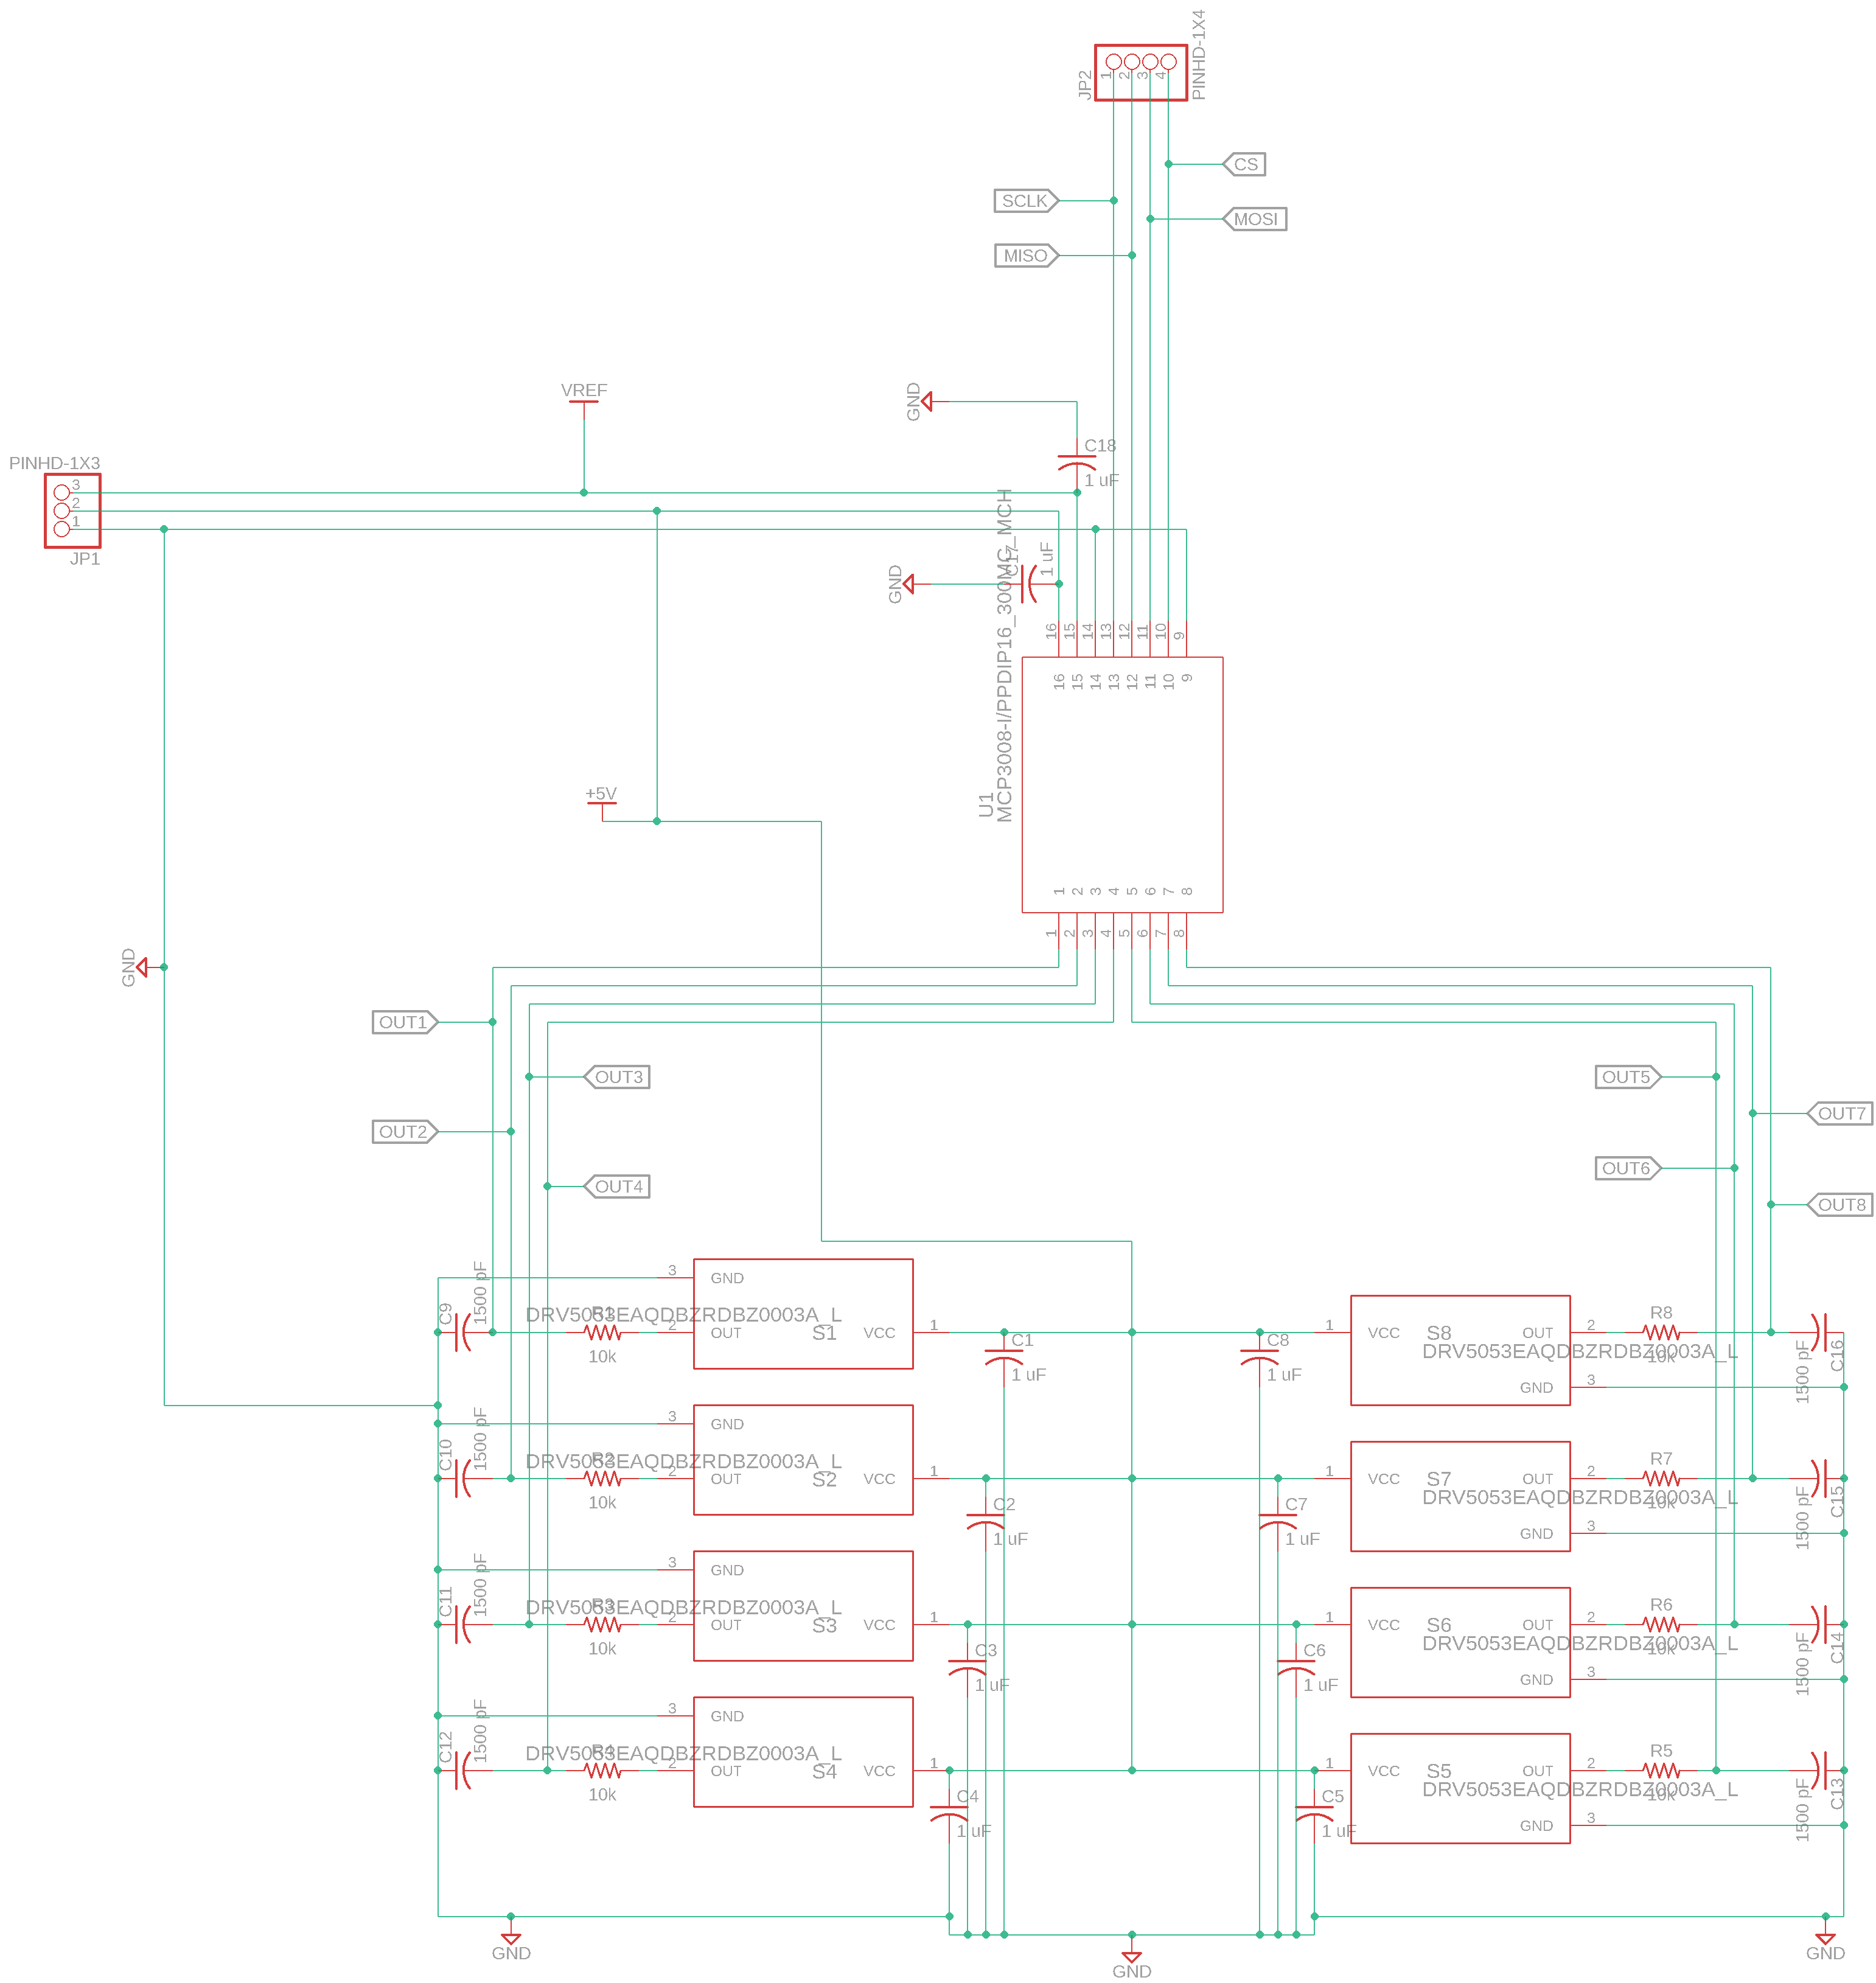
\includegraphics[width=\linewidth]{PCBSchematic.png}
  \caption{PCB Circuit Schematic}
  \label{pcbschematic}
\end{figure}
\begin{figure}[ht]
  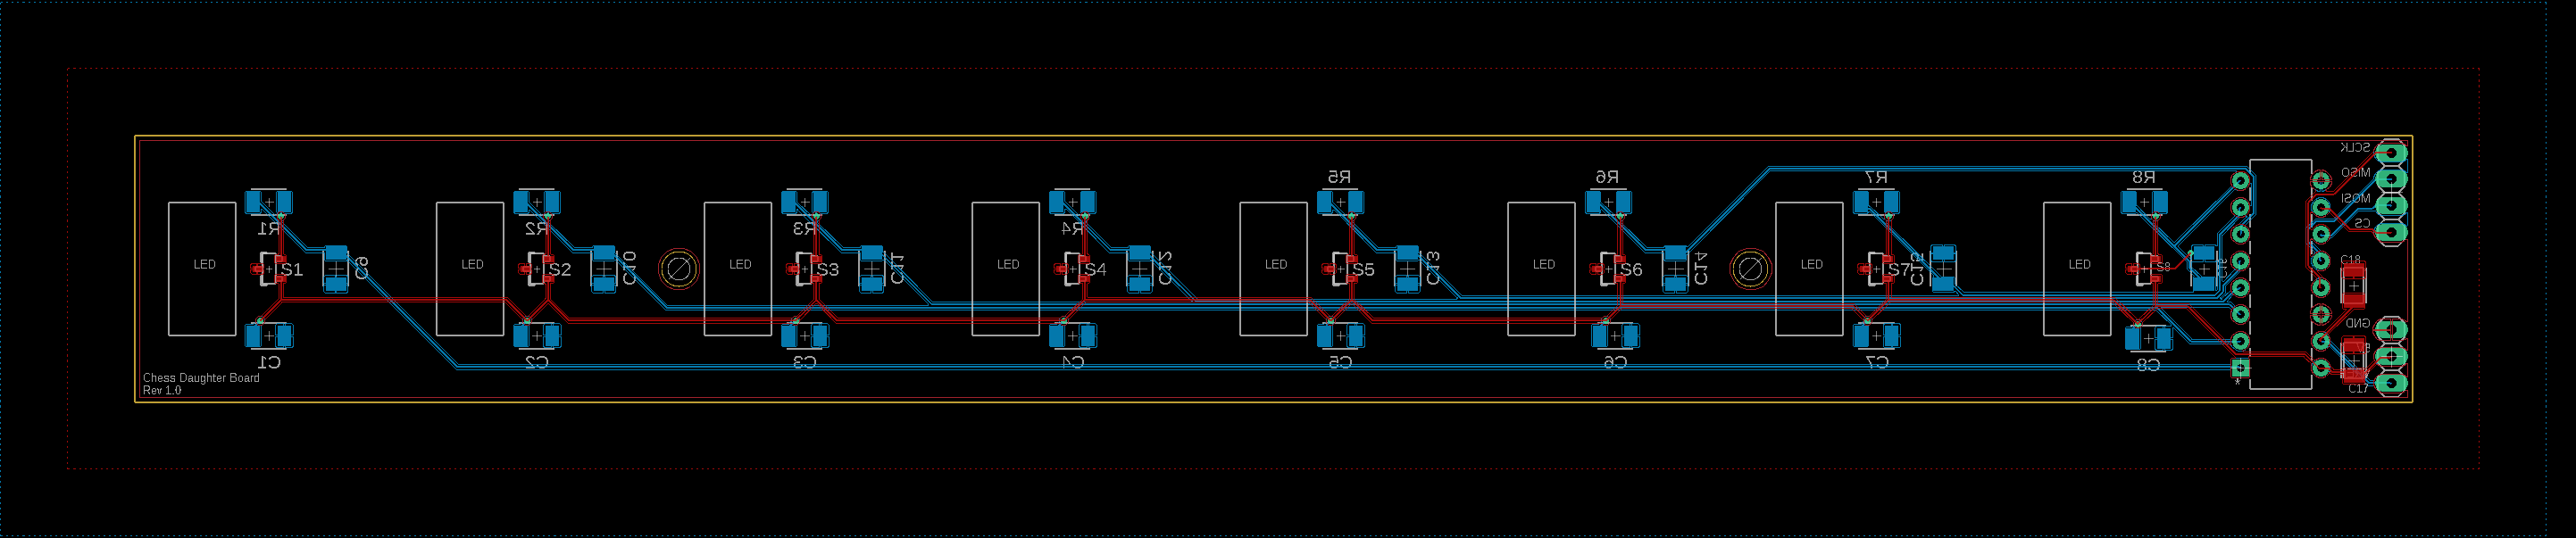
\includegraphics[width=\linewidth]{PCBLayout.png}
  \caption{PCB Design}
  \label{pcbdesign}
\end{figure}

\subsubsection{LEDs}
In order to display helpful information to the users, strip RGB LED lights were used. These lights were individually soldered together to create custom spacing and glued to the PCB to ensure that the lights were below each square. The Neopixel library was used to control the LEDs \cite{neopixel}. This was done through a single GPIO pin which transmitted serial data to the light strip as well as a connection to power and ground. These lights helped communicate different game states and information to the player. If all LEDs are off, the chess board is waiting for player interaction. Red LEDs indicate an error state and include light red spaces that must be changed to get to the last valid state. Lifting up a piece results in light blue lights indicating possible moves. Incomplete moves are marked by darker blue and show the player actions they must complete to finish the move. Finally, purple and pink LEDs were used to show the AI's move (moving pieces from and to spots respectively). These LEDs allowed players to see relevant information in real time as they play.

\subsubsection{Assembled Prototype}
With all the components in hand and all 8 PCBs soldered and validated, the design and assembly of the chessboard itself began. A 3D model of a chessboard was created that would house all of the physical components in Autodesk Maya and printed it using transparent PETG filament on a 3D printer. The housing was too big for the print area of the available 3D printers, so it was printed in two parts and glued together. Two total revisions of the housing were printed, and the second revision only needed an extra hole added for wiring purposes. Once the housing was printed, the eight PCBs were inserted and adhered to the board using mounting putty, which was used because the top layer of the chessboard was not thick enough to use the screw holes for mounting the PCBs. Then the breadboard was inserted containing the Pi Pico, as well as the buttons and display, and wired it all together using standard breadboard jumper cables. For the chess pieces, a free model was used and modified to have a hole in the base, and a magnet was glued in each piece. Please, see Fig.~\ref{boardtop}-\ref{boardbottom} for pictures of the final assembled prototype.
\begin{figure}[ht]
  \includegraphics[width=\linewidth]{boardTop.jpg}
  \caption{Top view of assembled chessboard}
  \label{boardtop}
\end{figure}
\begin{figure}[ht]
  \includegraphics[width=\linewidth]{boardBottom.jpg}
  \caption{Bottom view of assembled chessboard}
  \label{boardbottom}
\end{figure}
\subsection{Software}
\subsubsection{Micro Python Firmware}
The Pi Pico device consists of various libraries and code written in Micro Python to execute. Due to the architecture and design of the Pi Pico, running this firmware enables the Pi Pico to start running the code loaded onto it the moment it is connected to power through the Micro-USB port on the device. The Pi Pico's Micro-USB port has the dual-purpose of being the flashing port for loading on firmware, where IDEs and compilers such as VS Code and Thonny allow for easy debugging and programming purposes.

The firmware consisted of a top-level file, main.py, that was responsible for executing the main logic in a continuous while loop. It included references to other MicroPython files in its directory for executing the compartmentalized functions. These functions in the other MicroPython files consist of code for establishing connection to the WiFi network, parsing JSON objects to a 2D array, parsing 2D arrays to JSON objects, GET requests, POST requests, flags, buttons, LCD screen displays, and more.
When an individual is compiling the Pi Pico for their own use, it is important to change details specific to your own hotspot. This includes the IP, SSID (hotspot name), and password (hotspot password). This must also be done in the compiled Flutter project. This is to ensure a successful connection is established to the already running Android server. 

The Pi Pico firmware serves as the heart of the project, as well as the code. The firmware is responsible for telling the chessboard LEDs when to light up, how to detect chess pieces being moved, telling the player where they can move chess pieces, and so on. The Android application in communication with the Pi Pico serves as its guide to providing the Pi Pico its needed information based on the Pi Pico's detected chessboard changes and how the Pi Pico wants the Android device to handle them (such as when a new game starts or a specific game mode is selected. With proper communication established with the Android device, the Pi Pico is able to utilize the Android device to give the current state of the board and request what LEDs to turn on so that the next move can be shown or made.

Upon successful startup of the Android device and software, the web server that the Pi Pico Firmware requires to run is ready to be communicated with. Now, the Pi Pico can be connected to power. The LCD screen will turn on, prompting the user to select between the ``Play Friend'' and ``Play AI'' game modes. The user may use the designated up and down GPIO buttons to hover over their selection. Now, the user may press the designated select button to choose this game mode. This state operates under the assumption that all chessboard pieces are placed in their starting position and to begin a new game. The Pi Pico firmware conducts a POST request with a 2D array of the chess piece locations, as well as flag bits indicating a new game with the selected game mode to the Android device. The Pi Pico now sends a GET request to cycle back for the player to start.

The player picks up a piece. This triggers the specific ADC sensor for that chess piece tile to notice a change. Since a change occurred, all chessboard pieces and their locations are logged into the 2D array and sent in a POST request to the Android device. A GET request from the Pi Pico occurs, and the Android device answers back with a 2D array containing LEDs under which tiles the currently picked up piece can move to. When the piece is put down, the player presses the ``end of turn'' button to indicate they completed their move and the next player's turn begins. The GET, POST cycle continues, as this was a detected change in the chessboard. This cycle continues for the rest of the game. This logic varies between the ``Play Friend'' and ``Play AI'' game mode frameworks, as the ``Play AI'' game mode requires the player to move for the AI, so LEDs are sent back during their turn to indicate what piece and where to move this piece. Once a checkmate occurs, the LEDs under each tile are told to turn green. The ``reset'' button allows you to begin a new game and select your game mode once again. ``Play Friend'' game mode has a timer aspect that is displayed on the LCD screen to countdown while it is one player's turn. Just as what occurs in a checkmate, when a player runs out of time, all tiles flash green as this indicates game over.

\subsubsection{Android App}
The accompanying Android application is a flutter application, allowing for the potential of running this application on a variety of platforms including iOS and desktop. The app keeps track of all chess logic and includes a chess engine that tracks pieces, move history, board state, and all other statistics for the game. To create this, a standard chessboard class was created to allow for standard chess play and an extended integrated chessboard class was created to take input from the board and update both the visual and model representation of the board accordingly. Separate classes were also made for each type of chess piece in order to determine possible moves and state updating. These classes extended an abstract chesspiece class that outlined standard use cases for chess pieces including compiling possible moves, moving the actual piece in the game board, and determining data like string representations for each piece. To bring the chess pieces and chessboard logic together, a move class was made to keep track of piece information, ending coordinate locations, and special move determinations (such as if the move was part of a promotion, en passant, or castling move). The AI integration for the computer chess player was made using the stockfish library, which allows you to determine the best move based on a specific depth of search of the current chess state \cite{stockfish}. The app also allowed for a difficulty setting on the AI player (easy, medium, hard) which corresponded with the depth of search allowed for AI moves. See Fig.~\ref{chessapp} for example of starting state of the Android chess application.
\begin{figure}[ht]
  \includegraphics[width=\linewidth]{chessApp2.png}
  \caption{Chess Android Application}
  \label{chessapp}
\end{figure}
\subsubsection{Communication Protocols}
For communication between the Android Device and the Pi Pico, the team opted for a wireless local area network (WLAN) with a web server as the medium. The Android device is responsible for hosting, while the Pi Pico served as the user and client. Both devices established connection to the same mobile hotspot with the same ip on port 8080. The Android application is ran prior to the Pi Pico running its firmware in order to begin the hosting process and minimize HTTP request handling issues.

The Pi Pico, as the client and user, was solely responsible for contributing HTTP requests; such requests consisted of GET and POST. When a change to the chessboard, a POST request is sent with the updated array. This array is parsed into JSON, then sent in the POST request over to the Android device. The Android device runs listens asyncronously for incoming POST requests. Upon receiving a POST request from the Pi Pico, the Android device parses the received JSON object into an interpretable 2D, formatted array containing the location of all chess pieces and flags. This array's flag indices are checked to interpret what game mode and game state for the chess logic to apply. Upon chess logic applied (for either a new game, playing with a friend, or playing with the Stockfish API), the chess logic in the Android application sends its resulting 2D array to an LED handler. This handler is responsible for using the next chess moves possible and storing which LEDs to turn on in the 2D array for the Pi Pico to later retrieve in a GET request.

As previously mentioned, the stored 2D array is to indicate which LEDs to turn on. This 2D array stores the color of the LED in the index corresponding to the chess piece, just as it was previously used to tell where that piece was. In the meantime, the Pi Pico has already sent a GET requests that waits for the Android device to complete its new 2D LED array that it wants to GET. This occurs since every time the Pi Pico sends a POST request, a small loop of GET requests occur that waits for the Android device to answer back without an HTTP error code. This method of sending and receiving information has proven to be a very reliable, effective means of communication.


% You probably want subsections for tasks, testing and integration,
% management and communication, schedule and milestones, risk
% assessment, bill of materials (not necessarily in this order)


% \section{Results}
% \label{sec:results}
% 
% This section probably won't be in the proposal.


\section{Conclusion}
%Kenan wrote -- copied from the proposal tex%
The Smart Chess Board is a project designed to make chess fun and easier for everyone. It helps new players learn the game by showing possible moves and interactively teaching the rules. At the same time, it supports experienced players by recording games, tracking progress, and allowing them to play against an AI opponent.
The board combines physical hardware like sensors, LEDs, and buttons with digital software in a companion app. This mix of physical and virtual features makes learning and playing chess both engaging and accessible. For example:
LED lights show players where they can move their pieces.
Sensors detect when pieces are picked up or moved.
The app tracks game history and allows players to analyze their past matches.
AI gameplay means players can practice even without a partner.
This project was created to address problems associated with other smart chess boards, such as high costs and limited functionality. Despite using a 3D printer for specific components, modular components were used such as the Raspberry Pi Pico to keep the overall design affordable and practical. The Smart Chess Board is an innovative solution that balances functionality and accessibility.
This project also reflects great teamwork and careful planning:
Hardware specialists worked on the physical board, sensors, and electronics.
Software developers created the app and ensured smooth communication between the board and the app.
AI integration allowed players to improve their skills even when playing alone.
Finally, the Smart Chess Board makes chess more enjoyable for all players, easier to learn, and more engaging. Combining hands-on learning with advanced technology benefits beginners and experts alike.


\section*{Acknowledgment}

The authors would like to thank Romilly Cocking on GitHub for their MCP3008 MicroPython library. A considerable amount of time would have been spent writing a library and going over the documentation for the MCP3008 if not for their work \cite{cocking_pico_code_2023}. The authors would also like to thank Arjan Aswal and other contributors to the Stockfish Chess Engine along with its flutter package which allowed the board to determine possible AI moves at a variety of different difficulties \cite{stockfish}. Finally, the authors would like to thank Damien P. Geroge and Jim Mussared for the Neopixel MicroPython library which allowed the board to interface with the LED strip lights through out Raspbery Pi \cite{neopixel}.



\bibliographystyle{IEEEtran}  % IEEEtran -- needs IEEEtran.bst
% Balance the citations to equalize the columns manually
% \balance
\bibliography{proposal}

\end{document}


% LocalWords:  Eqn df
